% Étape 1 : choix de l'architecture. Sources : notebooks/01_architectures.ipynb, results/etape1_*.

\section{Choix de l'architecture}
\label{sec-architectures}

Le réseau doit remplacer Fourier pendant la calibration : il doit donc être à la fois précis et nettement plus
rapide que Fourier. Cette section choisit sa taille, c'est-à-dire le nombre de couches cachées et de neurones par
couche.

\subsection{Protocole}
\label{sec-archi-protocole}

Le réseau est un perceptron multicouche : il prend les 5 paramètres de Heston (normalisés) et renvoie les 88
volatilités de la grille ; la couche de sortie est linéaire, puisqu'il s'agit d'une régression. La perte est
l'erreur quadratique moyenne, calculée uniquement sur les points connus de chaque surface : les points manquants
(NaN, voir \cref{sec-donnees}) sont ignorés, ce qui permet de garder toutes les surfaces.

Nous comparons 10 architectures : 2, 4 ou 6 couches cachées de 32, 128 ou 512 neurones, plus le réseau
$4\times30$ de \citet{horvath2021}, qui sert de référence. Seule l'architecture change : toutes sont entraînées
de la même façon, avec Adam, l'initialisation de He et l'activation ELU, pendant 200 époques avec des lots de 32
surfaces, sur le même découpage des données (\SI{80}{\percent} entraînement, \SI{10}{\percent} validation,
\SI{10}{\percent} test). Nous gardons les poids de la meilleure époque sur la validation.

Chaque architecture est entraînée 5 fois, avec 5 graines différentes, sur exactement le même découpage des
données : la graine ne change que l'initialisation des poids et l'ordre des lots. Les écarts-types mesurent donc
la variabilité de l'entraînement lui-même, pas celle des données. Les choix se font sur la validation ; le test ne
sert qu'aux chiffres finaux. L'erreur est l'écart absolu moyen entre la volatilité prédite et la vraie, en points
de base ($1\pb = 0{,}01$ point de volatilité).

\subsection{Taux d'apprentissage}
\label{sec-archi-taux}

Avant de comparer les architectures, nous fixons le taux d'apprentissage d'Adam sur le réseau de référence
$4\times30$, avec trois valeurs (\cref{fig-taux}). Avec $10^{-2}$, l'apprentissage est instable : l'erreur de
validation oscille et atteint \num{14.3}\pb. Avec $10^{-4}$, il est trop lent : \num{9.2}\pb\ après 200 époques,
et le réseau progresse encore. Nous retenons $10^{-3}$ (\num{7.6}\pb), utilisé dans toute la suite.

\begin{figure}[H]
  \centering
  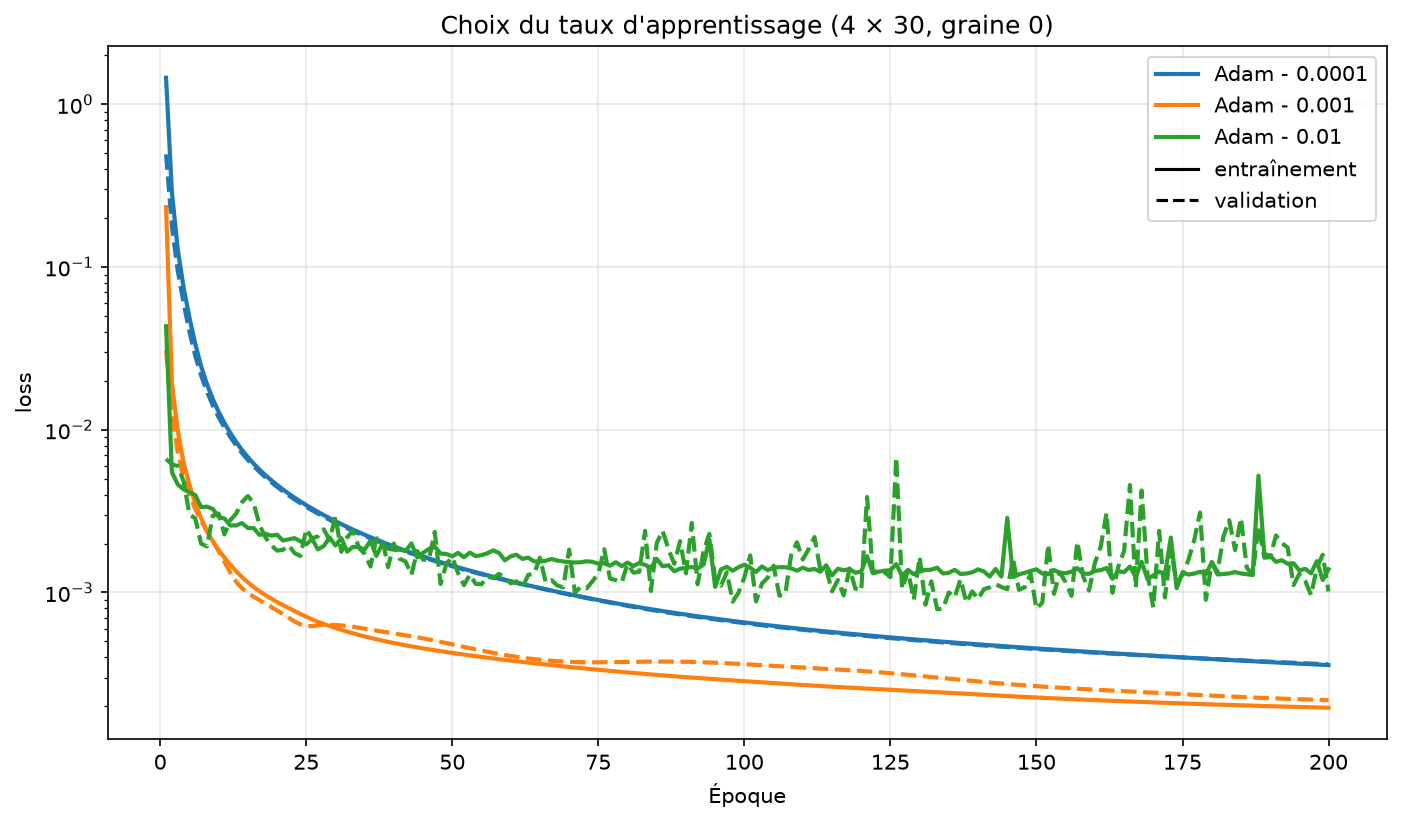
\includegraphics[width=0.8\textwidth]{etape1_taux}
  \caption{Perte d'entraînement (trait plein) et de validation (pointillés) du réseau $4\times30$ pour trois taux
  d'apprentissage.}
  \label{fig-taux}
\end{figure}

\subsection{Précision}
\label{sec-archi-precision}

Le \cref{tab-archi} donne les erreurs des 10 architectures et la \cref{fig-courbes} leurs courbes
d'apprentissage.

Augmenter la taille du réseau n'améliore pas la précision au-delà d'un certain point. Les réseaux de 512 neurones
sur 4 et 6 couches sont moins précis que des réseaux bien plus petits, et instables d'une graine à l'autre : le
$6\times512$ fait \num{14.8} $\pm$ \num{11.5}\pb. Leur perte de validation reste au-dessus des autres et oscille
fortement (\cref{fig-courbes}), signe qu'avec le même taux d'apprentissage, ces grands réseaux sont plus difficiles
à entraîner.

Ajouter des couches n'aide pas non plus. À largeur constante de 128 neurones, les réseaux plus profonds font même
un peu moins bien (\num{5.09},
\num{5.45} et \num{5.90}\pb\ pour 2, 4 et 6 couches). À 32 neurones, toutes les profondeurs se valent (de
\num{6.5} à \num{7.6}\pb), et le réseau de \citet{horvath2021} se situe au même niveau (\num{6.75}\pb).

Les erreurs de validation et de test sont très proches pour toutes les architectures : l'écart absolu moyen est
de \num{0.04}\pb, et ne dépasse jamais \num{0.2}\pb. Les deux jeux sont pourtant distincts et évalués séparément :
leurs erreurs maximales diffèrent nettement (pour le $2\times128$, graine 0 : \num{112}\pb\ en validation contre
\num{129}\pb\ en test). Cette proximité s'explique par leur taille : chacun contient \num{5000} surfaces, soit
environ \num{430000} volatilités connues tirées de la même distribution, ce qui stabilise l'estimation de l'erreur
moyenne, même si les volatilités d'une même surface ne sont pas indépendantes. À la meilleure époque, la perte
d'entraînement reste du même ordre que la perte de validation : nous ne voyons pas de surapprentissage marqué.
La meilleure époque est le plus souvent entre 170 et 200 :
avec un budget plus long, les réseaux progresseraient encore un peu.

\begin{table}[H]
  \centering
  \caption{Erreur moyenne (pb, moyenne $\pm$ écart-type sur 5 graines), erreur maximale moyenne sur le test,
  nombre de paramètres, temps de réponse pour une surface et gain par rapport à Fourier (\SI{2.29}{\ms}).
  Les erreurs de validation et de test diffèrent de moins de 0,2 pb, d'où des valeurs identiques une fois
  arrondies.}
  \label{tab-archi}
  \small
  \begin{tabular}{lcccrrr}
    \toprule
    Architecture & Validation & Test & Erreur max & Paramètres & Temps (ms) & Gain \\
    \midrule
    $2\times512$          & $4{,}67 \pm 0{,}42$   & $4{,}67$  & 173 & \num{310872}  & \num{0.39}  & \num{5.9} \\
    $\mathbf{2\times128}$ & $\mathbf{5{,}09 \pm 0{,}52}$ & $\mathbf{5{,}09}$ & 161 & \num{28632} & \num{0.028} & \num{83} \\
    $4\times128$          & $5{,}45 \pm 0{,}33$   & $5{,}45$  & 145 & \num{61656}   & \num{0.051} & \num{45} \\
    $6\times128$          & $5{,}90 \pm 0{,}26$   & $5{,}89$  & 132 & \num{94680}   & \num{0.074} & \num{31} \\
    $4\times32$           & $6{,}52 \pm 1{,}07$   & $6{,}49$  & 164 & \num{6264}    & \num{0.023} & \num{99} \\
    $4\times30$ (Horvath) & $6{,}75 \pm 0{,}67$   & $6{,}77$  & 150 & \num{5698}    & \num{0.023} & \num{100} \\
    $6\times32$           & $6{,}75 \pm 0{,}78$   & $6{,}78$  & 145 & \num{8376}    & \num{0.032} & \num{72} \\
    $2\times32$           & $7{,}63 \pm 0{,}86$   & $7{,}64$  & 249 & \num{4152}    & \num{0.020} & \num{113} \\
    $4\times512$          & $7{,}90 \pm 1{,}20$   & $7{,}90$  & 145 & \num{836184}  & \num{1.18}  & \num{1.9} \\
    $6\times512$          & $14{,}8 \pm 11{,}5$   & $14{,}8$  & 241 & \num{1361496} & \num{2.11}  & \num{1.1} \\
    \bottomrule
  \end{tabular}
\end{table}

\begin{figure}[H]
  \centering
  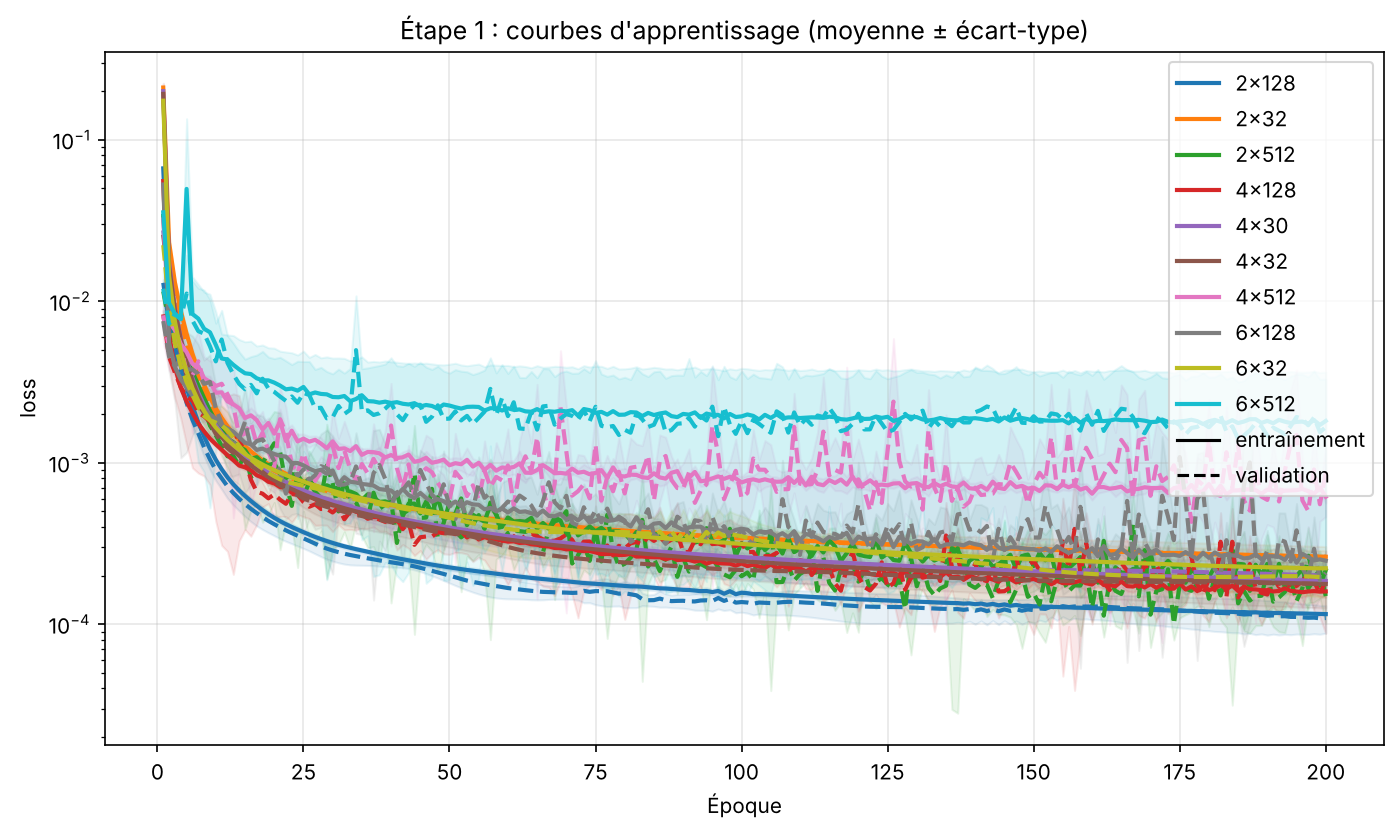
\includegraphics[width=\textwidth]{etape1_courbes}
  \caption{Courbes d'apprentissage des 10 architectures : moyenne $\pm$ écart-type sur 5 graines, entraînement en
  trait plein et validation en pointillés.}
  \label{fig-courbes}
\end{figure}

\subsection{Temps de réponse et choix}
\label{sec-archi-choix}

Le temps de réponse est mesuré pour une seule surface, sur la même machine que Fourier, au repos. Pour une seule
surface, un appel à Keras ajoute environ \SI{3}{\ms} de frais fixes, plus que Fourier lui-même : nous mesurons donc
la prédiction refaite en numpy, couche par couche, à partir des poids du réseau. Ce temps ne dépend que de la
taille du réseau, et grandit vite avec la largeur : de \SI{0.02}{\ms} pour les réseaux de 32 neurones à
\SI{2.1}{\ms} pour le $6\times512$, presque autant que Fourier.

Le seuil de vitesse a été fixé en regardant uniquement les temps, avant de comparer les précisions : le réseau doit
être au moins 10 fois plus rapide que Fourier. Il élimine les trois réseaux de 512 neurones, entre 1,1 et
5,9 fois plus rapides seulement (\cref{fig-erreur-temps}). Pour choisir parmi les 7 architectures restantes, nous
partons de la plus précise sur la validation ; comme l'écart entre deux architectures reste faible au regard de la
variabilité observée entre les graines, nous retenons la plus rapide de celles qui sont à moins d'un écart-type
d'elle. La plus précise est le $2\times128$ (\num{5.09} $\pm$ \num{0.52}\pb) ; le $4\times128$ est à moins d'un
écart-type (\num{5.45}\pb), mais presque deux fois plus lent.

Nous retenons donc le $2\times128$ : \num{5.09}\pb\ sur la validation et sur le test, 83 fois plus rapide que
Fourier. Il fait mieux que l'architecture $4\times30$ de \citet{horvath2021}, entraînée avec notre protocole
(\num{6.75}\pb), pour un temps de réponse comparable.

\begin{figure}[H]
  \centering
  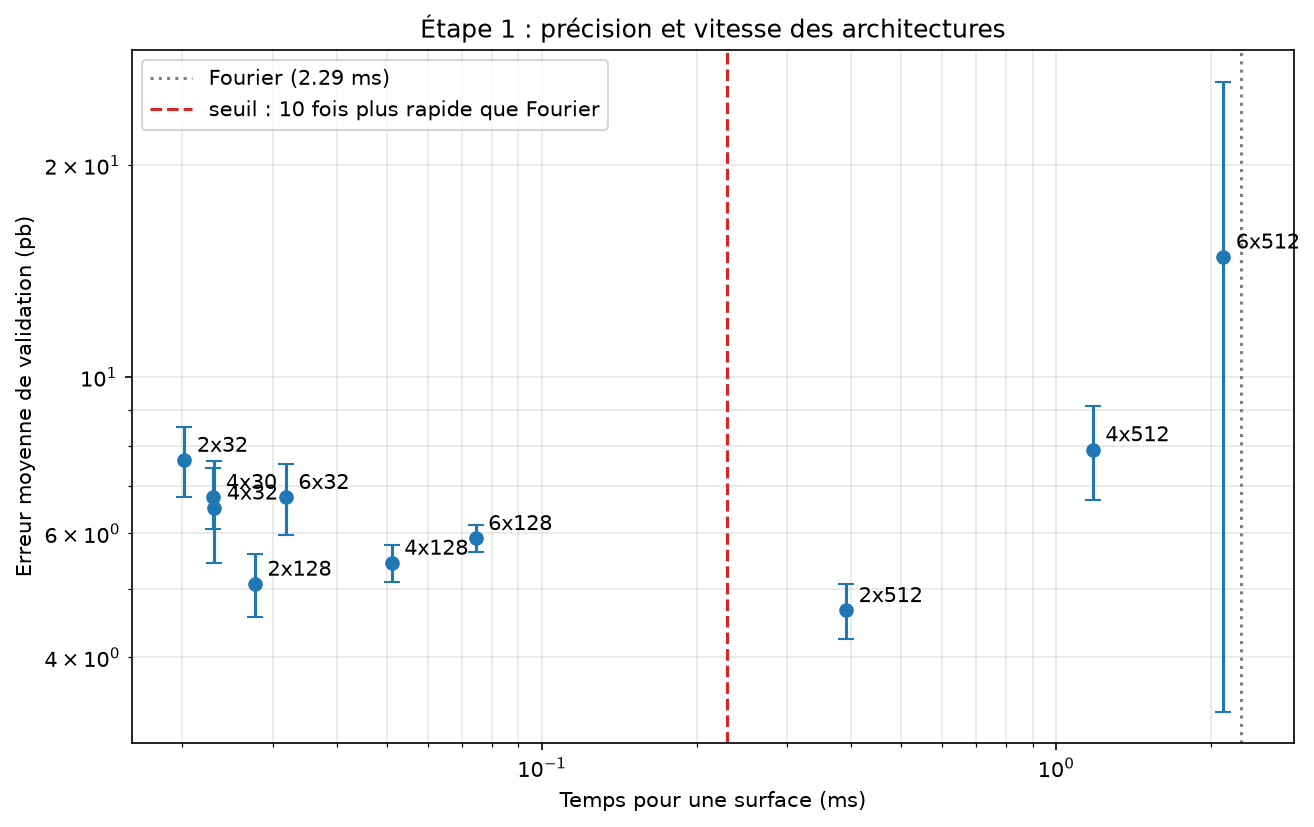
\includegraphics[width=0.85\textwidth]{etape1_erreur_temps}
  \caption{Erreur de validation (moyenne $\pm$ écart-type sur 5 graines) en fonction du temps de réponse pour une
  surface. Ligne pointillée grise : Fourier ; ligne rouge : seuil de vitesse (10 fois plus rapide que Fourier).}
  \label{fig-erreur-temps}
\end{figure}
